% !TeX spellcheck = en_US
\documentclass{article}

\usepackage{amsmath}
\usepackage{amssymb}
\usepackage[english]{babel}
\usepackage{booktabs}
\usepackage{color}
\usepackage{float}
\usepackage[margin=1in,includefoot]{geometry}
\usepackage{graphics}
\usepackage{graphicx}
\usepackage{wrapfig}
\usepackage[hidelinks]{hyperref}
\usepackage{lipsum}
\usepackage{listings}

\usepackage[numbers,sort&compress]{natbib}
\usepackage{subcaption}
\usepackage{tabularx}
\usepackage[normalem]{ulem}
\usepackage{url}

\useunder{\uline}{\ul}{}

\usepackage[usenames,dvipsnames]{xcolor}



% Header and Footer Stuff
\usepackage{fancyhdr}
\pagestyle{fancy}
\fancyhead{}
\fancyfoot{}
\fancyfoot[R]{\thepage}
\renewcommand{\headrulewidth}{0pt}
\renewcommand{\footrulewidth}{0pt}




\definecolor{dkgreen}{rgb}{0,0.6,0}
\definecolor{gray}{rgb}{0.5,0.5,0.5}
\definecolor{mauve}{rgb}{0.58,0,0.82}

% package to highlight code
\lstset{
 language=C++,
 aboveskip=3mm,
 belowskip=3mm,
 showstringspaces=false,
 columns=flexible,
 basicstyle={\small\ttfamily},
 numbers=none,
 numberstyle=\tiny\color{gray},
 keywordstyle=\color{blue},
 commentstyle=\color{dkgreen},
 stringstyle=\color{mauve},
 breaklines=true,
 breakatwhitespace=true,
 tabsize=3
}

\begin{document}

\begin{titlepage}
	\begin{center}
	\begin{align*}
	
\includegraphics[height=1.75in]{logo.png}
	\end{align*}
	
	\line(1,0){300}\\
	[0.25in]Augmented Reality
	\huge{\bfseries }\\
	[2mm]
	\line(1,0){200}\\
	[1.5cm]
	\textsc{\LARGE Panorama Stitching }\\
	[0.75cm]
	\textsc{\Large Final Year}\\
	[6cm]	
	\end{center}
	
	\begin{flushright}
	\textsc{\large Alexandru Sulea\\
	D Stream\\
	\#12315152\\
	30 April 2017\\}
	\end{flushright}
	
\end{titlepage}


%Table of Contents Stuff%
\tableofcontents
%\listoffigures
%\addcontentsline{toc}{section}{List of Figures}
\listoftables
%\addcontentsline{toc}{section}{List of Tables}

\thispagestyle{empty}
\cleardoublepage
\pagenumbering{arabic}
\setcounter{page}{1}

\pagebreak




\section{Introduction}\label{sec:overview}




The project work is done in opencv3 which is the newest version of opencv. The newer version has more updated functions, especially for 3D processing and point cloud processing. However due to copyright issues with stitching and many other algorithms, the most powerful and useful parts of the opencv package have been split up into a different repository for opencv3. Therefore to get the full opencv3 package , one needs to use cmake and build opencv3 with the include libraries in opencv contrib. A vanilla build is relatively simple to do but if attempting to use some of the non-free algorithms, the process becomes extensively more difficult.

For this project, the initial panorama stitching was chosen due to the fact that the only other projects that were being made were filters and possibly feature detection. In an effort to explore and learn more about stitching and panoramas the default project was chosen.

Initially image stitching was performed, this takes two images and seeks to stitch them together using common features from both the images.


To build on this early success, video panorama stitching was attempted where the frames from a video are taken and a panorama is constructed from them if the frames meet the panorama stitching requirement.\\
This process has been a little more complicated due to the fact that not all panorama videos move at the same speed or even in a linear motion capturing the scene from one side.\\
After some modifications though this was shown to work reliably across many frames. In practice only 2 frames were taken, in theory though this can be further expanded where the process will continually compare the constructed panorama against upcoming frames to check if the panorama can be further expanded.

Lastly haar cascades were used to detect the eyes and face and draw a square around them. The images were first analysed through haar cascades for faces and then afterwards the iamges were combined togeather to create a panorama which can detect people. 


The overall goal of the project was to create a system which could optimize current security systems by no just showing camera feeds on multiple screens.

Perhaps a more advanced system could allow for panorama stitching across multiple screens while detecting people. \\
Lastly perhaps the amalgamated video feeds could then create a 3d representation of the area the cameras are survailing, this has the added benefit of 3d location of subjects in a scene.\\


The program was initially attempted in c++ on a windows system, due to the large amount of package managing involved as well as the fact that many packages are no longer supported , the decision was made to change from c++ to python and from windows to ubuntu. 
The largest part of migrating the project to python and ubuntu was the fact that while vtk is still maintained for windows distributions, any other extra non-free modules of opencv have lost support for windows distributions.
\pagebreak

\section{Theoretical background}\label{sec:overview}
The theoretical implementation of panorama stitching follows that of the stitching pipeline.\\ 
An image is first read into the program , then the image quality is minimized, this is because of processing optimization, decreasing the quality of the picture may mean losing some accuracy, but as long as the image has 4 similar features with its neighbor than this loss in quality can be accepted.
The next step is finding the features between multiple images, this can be done through a variety of feature detection algorithms found in opencv.

\begin{figure}[H]
	\centering
	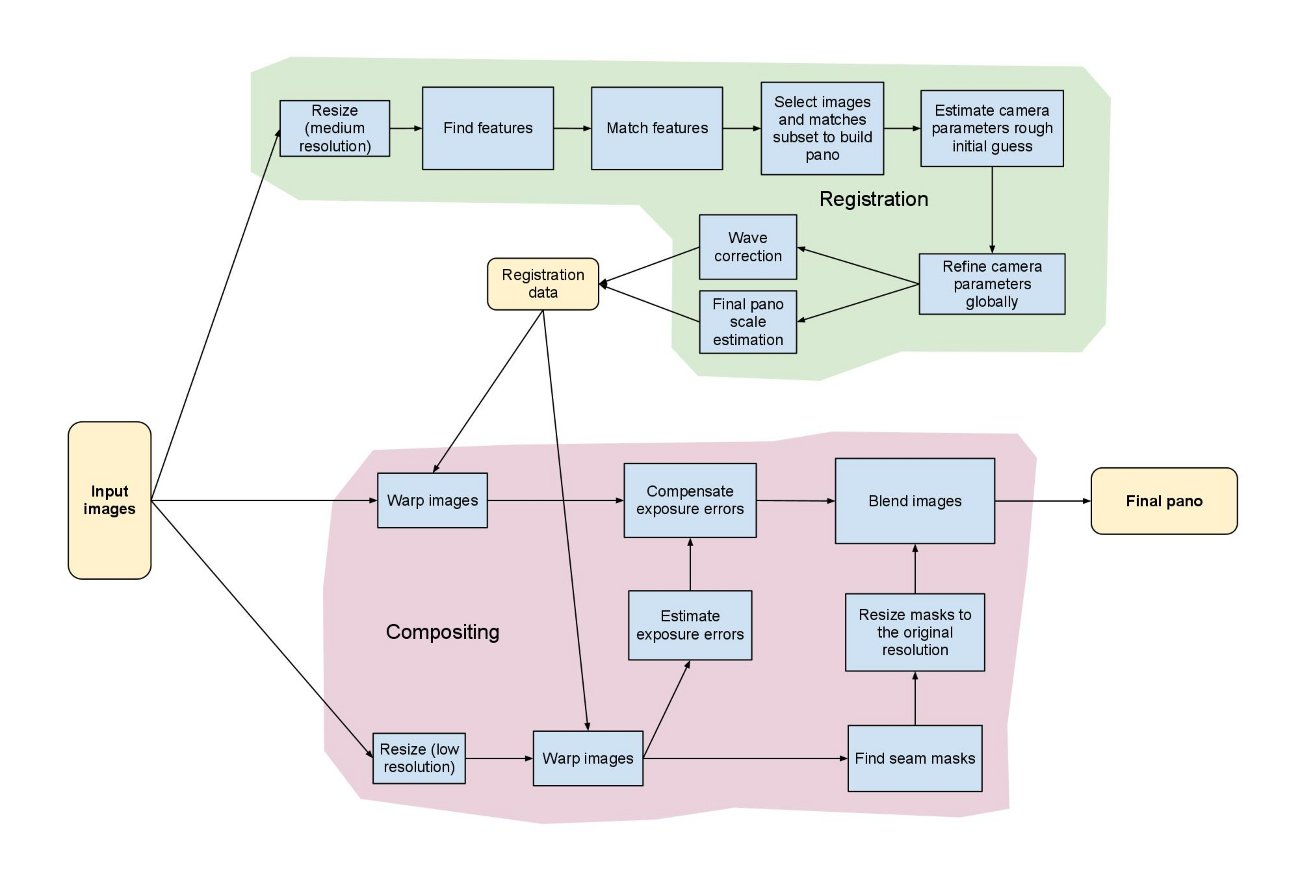
\includegraphics[width=10cm]{sp.jpg}
	 \caption{http://docs.opencv.org/3.0-beta/doc/py\_tutorials/py\_feature2d/py\_matcher/py\_matcher.html}
\end{figure}





But the ones we are most concerted are the feature detection algorithms which can then be used in homography \cite{ref:homo} for feature matching. Thus algorithms such as SIFT , FLANN and ORB can be used to detect features which will then be given a corresponding 2D point space.


http://docs.opencv.org/2.4/modules/stitching/doc/introduction.html

The next step is significantly more difficult as after the features are found and the matching keypoints returned, the features have to be matched. This is somewhat dependent on the type of matching that is used, but is similar enough across that one can switch flann for sift and the matches are still made. However, the accuracy may vary greatly depending on the type of feature finding and feature matching algorithms used. One the samples in this project, it is found that the most accurate while maintaining speed in video panoramic stitching was to detect using sift and match using flann.\\

After the features are found and matched, then they must be stitched together. The two images are drawn together by way of finding out the most common feature in the left and right image and then blending the two images together using the common points as an anchor for where to merge the images.


If the images are not taken on the same linear plane , then the images must be either warped or de-warped, enlarged or decreased so as to fit the pre-requisites of constructing a panoramic image.
\pagebreak
\section{Implementation}\label{sec:overview}
from pyimagesearch.panorama import Stitcher
import numpy as np\\
from numpy import pi,sin,cos,mgrid\\
import argparse\\
import imutils\\
import cv2\\

from matplotlib import pyplot as plt\\
from matplotlib import image as mpimg\\
from PIL import Image\\


These are the normal pre-requisites for panorama stitching ,cv2 for the opencv3 packages , imultis for grayscale and other image manipulations and numpy along wit.

cap = cv2.VideoCapture('video2.mp4', 0)\\

while (cap.isOpened()):\\
		key = cv2.waitKey1
frameId = int(round(cap.get(1)))
ret, frame = cap.read()


if frameId \% multiplier == 0:\\
if count $>$ 2:\\
frame = cv2.resize(frame, (0, 0), fx=0.5, fy=0.5)\\

stitcher = Stitcher()\\
(result, vis) = stitcher.stitch([frame, prev], showMatches=True)\\
cv2.imshow('result', result)\\
cv2.imshow('vis', vis)\\

(result2, vis2) = stitcher.stitch([prev\_result, frame], showMatches=True)\\

cv2.imshow('result2', result2)\\
cv2.imshow('vis2', vis2)\\
prev\_result= result\\


prev=frame\\

count += 1\\

break\\
cap.release()



The video is loaded in to the program and the frames are passed through. After verifying that the frames are ok, the video skips every 5 seconds. This is so as to allow the video frames to be far enough from each other to stitch a meaningful panorama as well as that less frames being stitched together means a faster processing speed for other jobs.

The prev and current frame are then loaded into the stitcher function. after the frames have been stitched together result will display the stitched panorama while vis will display the keypoints in both frames. 

The code is the exact same for image stitching but without the passing through multiple frames, as this is not required.
The code was mainly built from the opencv python basic panorama stitching tutorial.  \cite{ref:pc1}

The stitching pipeline Stitch() has 3 distinct functions. They are firstly to load the pictures in  and using flann or sift or brute force discern the keypoins in the images. 
After the keypoints have been localised then they are warped, so as to allow for any images that were not taken in a strict linear fashion. \\
Lastly the keypoints are drawn and stitched into the resulting panoramic and keypoint views which will show the panorama and the keypoint locations.



In option 3 of the program,the program searches for faces using the haar cascades for face and eye detection before stitching is initialized .The code for face detection being built on from the tutorial found at the opencv pages.\cite{ref:fd}
The face and eye detection are taken from xml files within opencv\_contrib. After the image is read in the haar cascades compare they're settings to the image in a effort to detect any eyes or faces. If a face or eyes is detected then the output image will have squares drawn corresponding in the positions where opencv believes to have detected eyes or faces.




\section{Experiments}\label{sec:overview}

A multitude of panorama stitchings were explored, such as using SIFT and RANSAC as well as BruteForce. One of the main factors which prevent good results will be the point at which the picture is sampled and the amount of light in the scene.

The point at which pictures are taken to be stitched is very important. A minimum amount of overlap is always required so as to be able to discern the points at which the stitching will take place. Overlap is also important for homography so as to discern at what angle the picture was taken and how it fits into the larger panoramic mosaic.


\begin{figure}[H]
	\centering
	
\includegraphics[width=4cm]{face1.jpg}

\includegraphics[width=4cm]{face2.jpg}

\includegraphics[width=4cm]{face3.jpg}
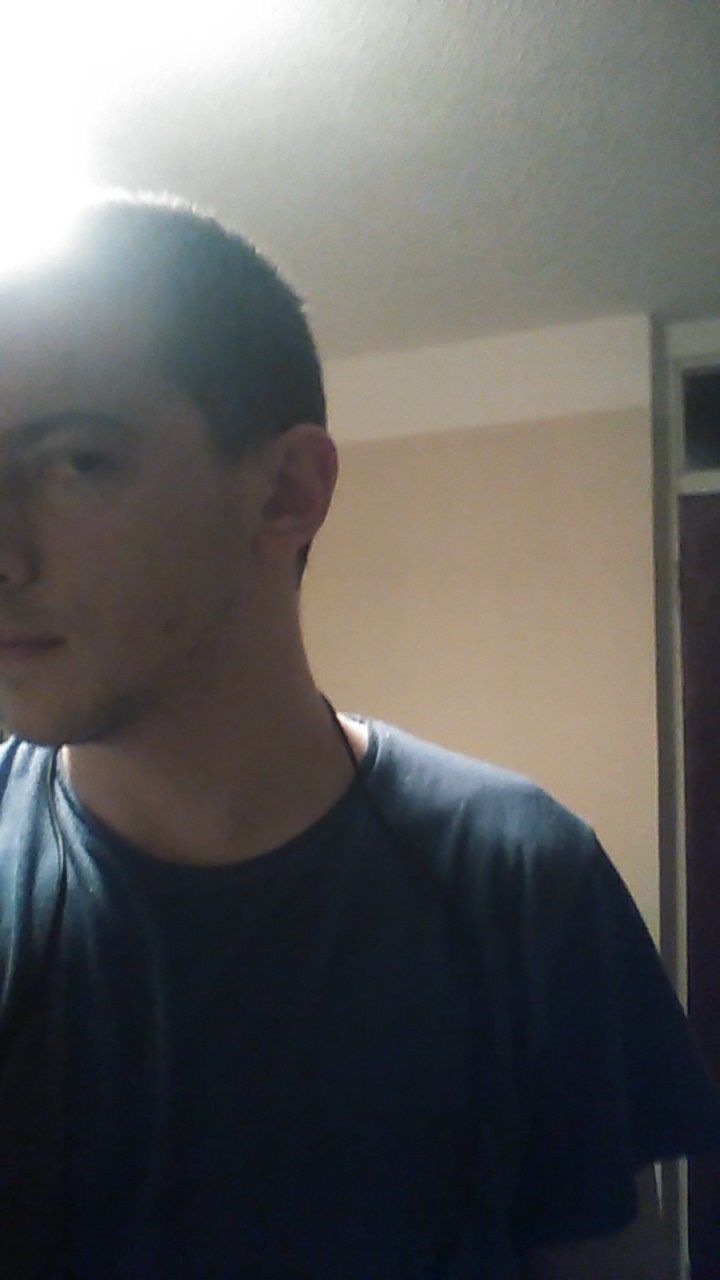
\includegraphics[width=4cm]{face4.jpg}
	
\end{figure}


The above pictures are a good example of this as though they may be stitched together, the fact that the light is shining directly into the camera means that haar cascades cannot work and thus the face or the eyes cannot be detected.\\
Therefore it is always recommended that when performing panorama stitching that the pictures be taken horizontally and also to avoid places of low or high light intensity as much as possible.

\begin{figure}[H]
	\centering
	
\includegraphics[width=4cm]{img5.jpg}
	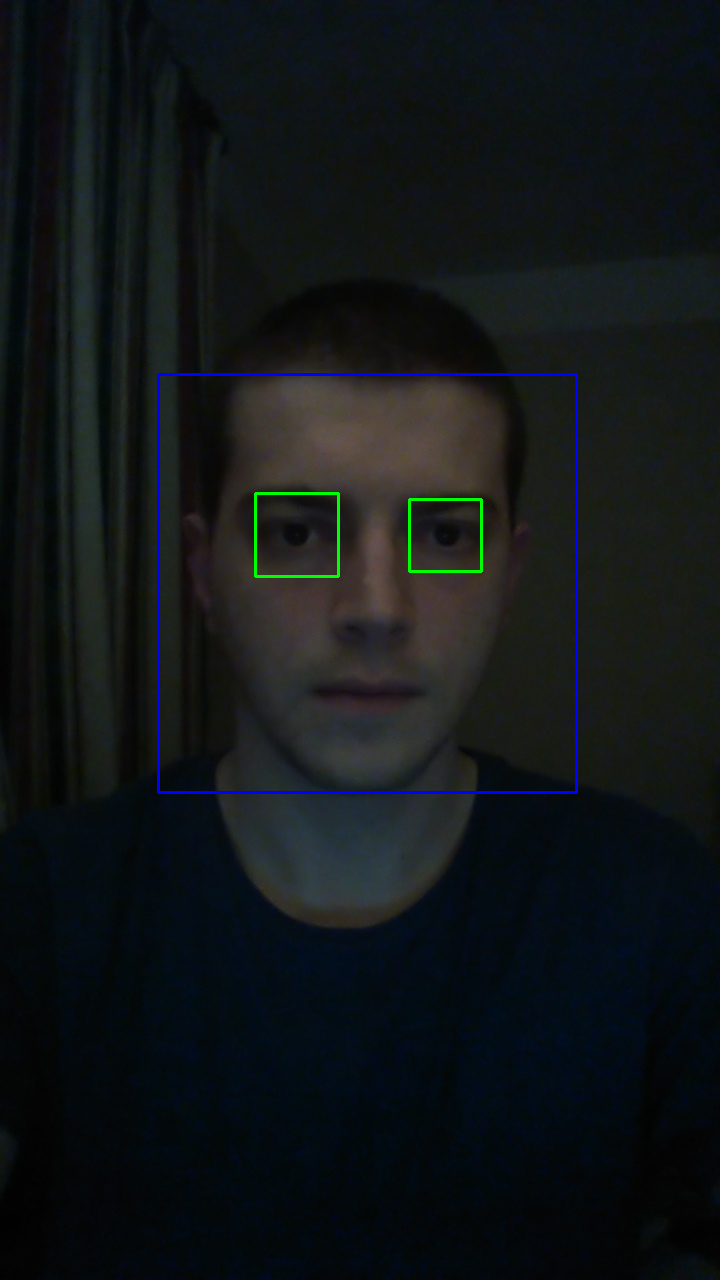
\includegraphics[width=4cm]{img55.png}
	
\end{figure}

While face detection will sometimes fail, eyed detection can still work in relatively low light. As shown in the figures above, after the light source was dimmed down the haar cascades gained more accuracy.\\


\section{Discussion of Results}\label{sec:overview}

\subsection{Part 1}\label{sec:overview}

As discussed previously, 2 colored images are taken and read into the program. these images must be overlapping and must be taken from the same direction. Thus 2 overlapping images from 2 distinctively alternating different sides would not render a good panorama.
\begin{figure}[H]
	\centering
	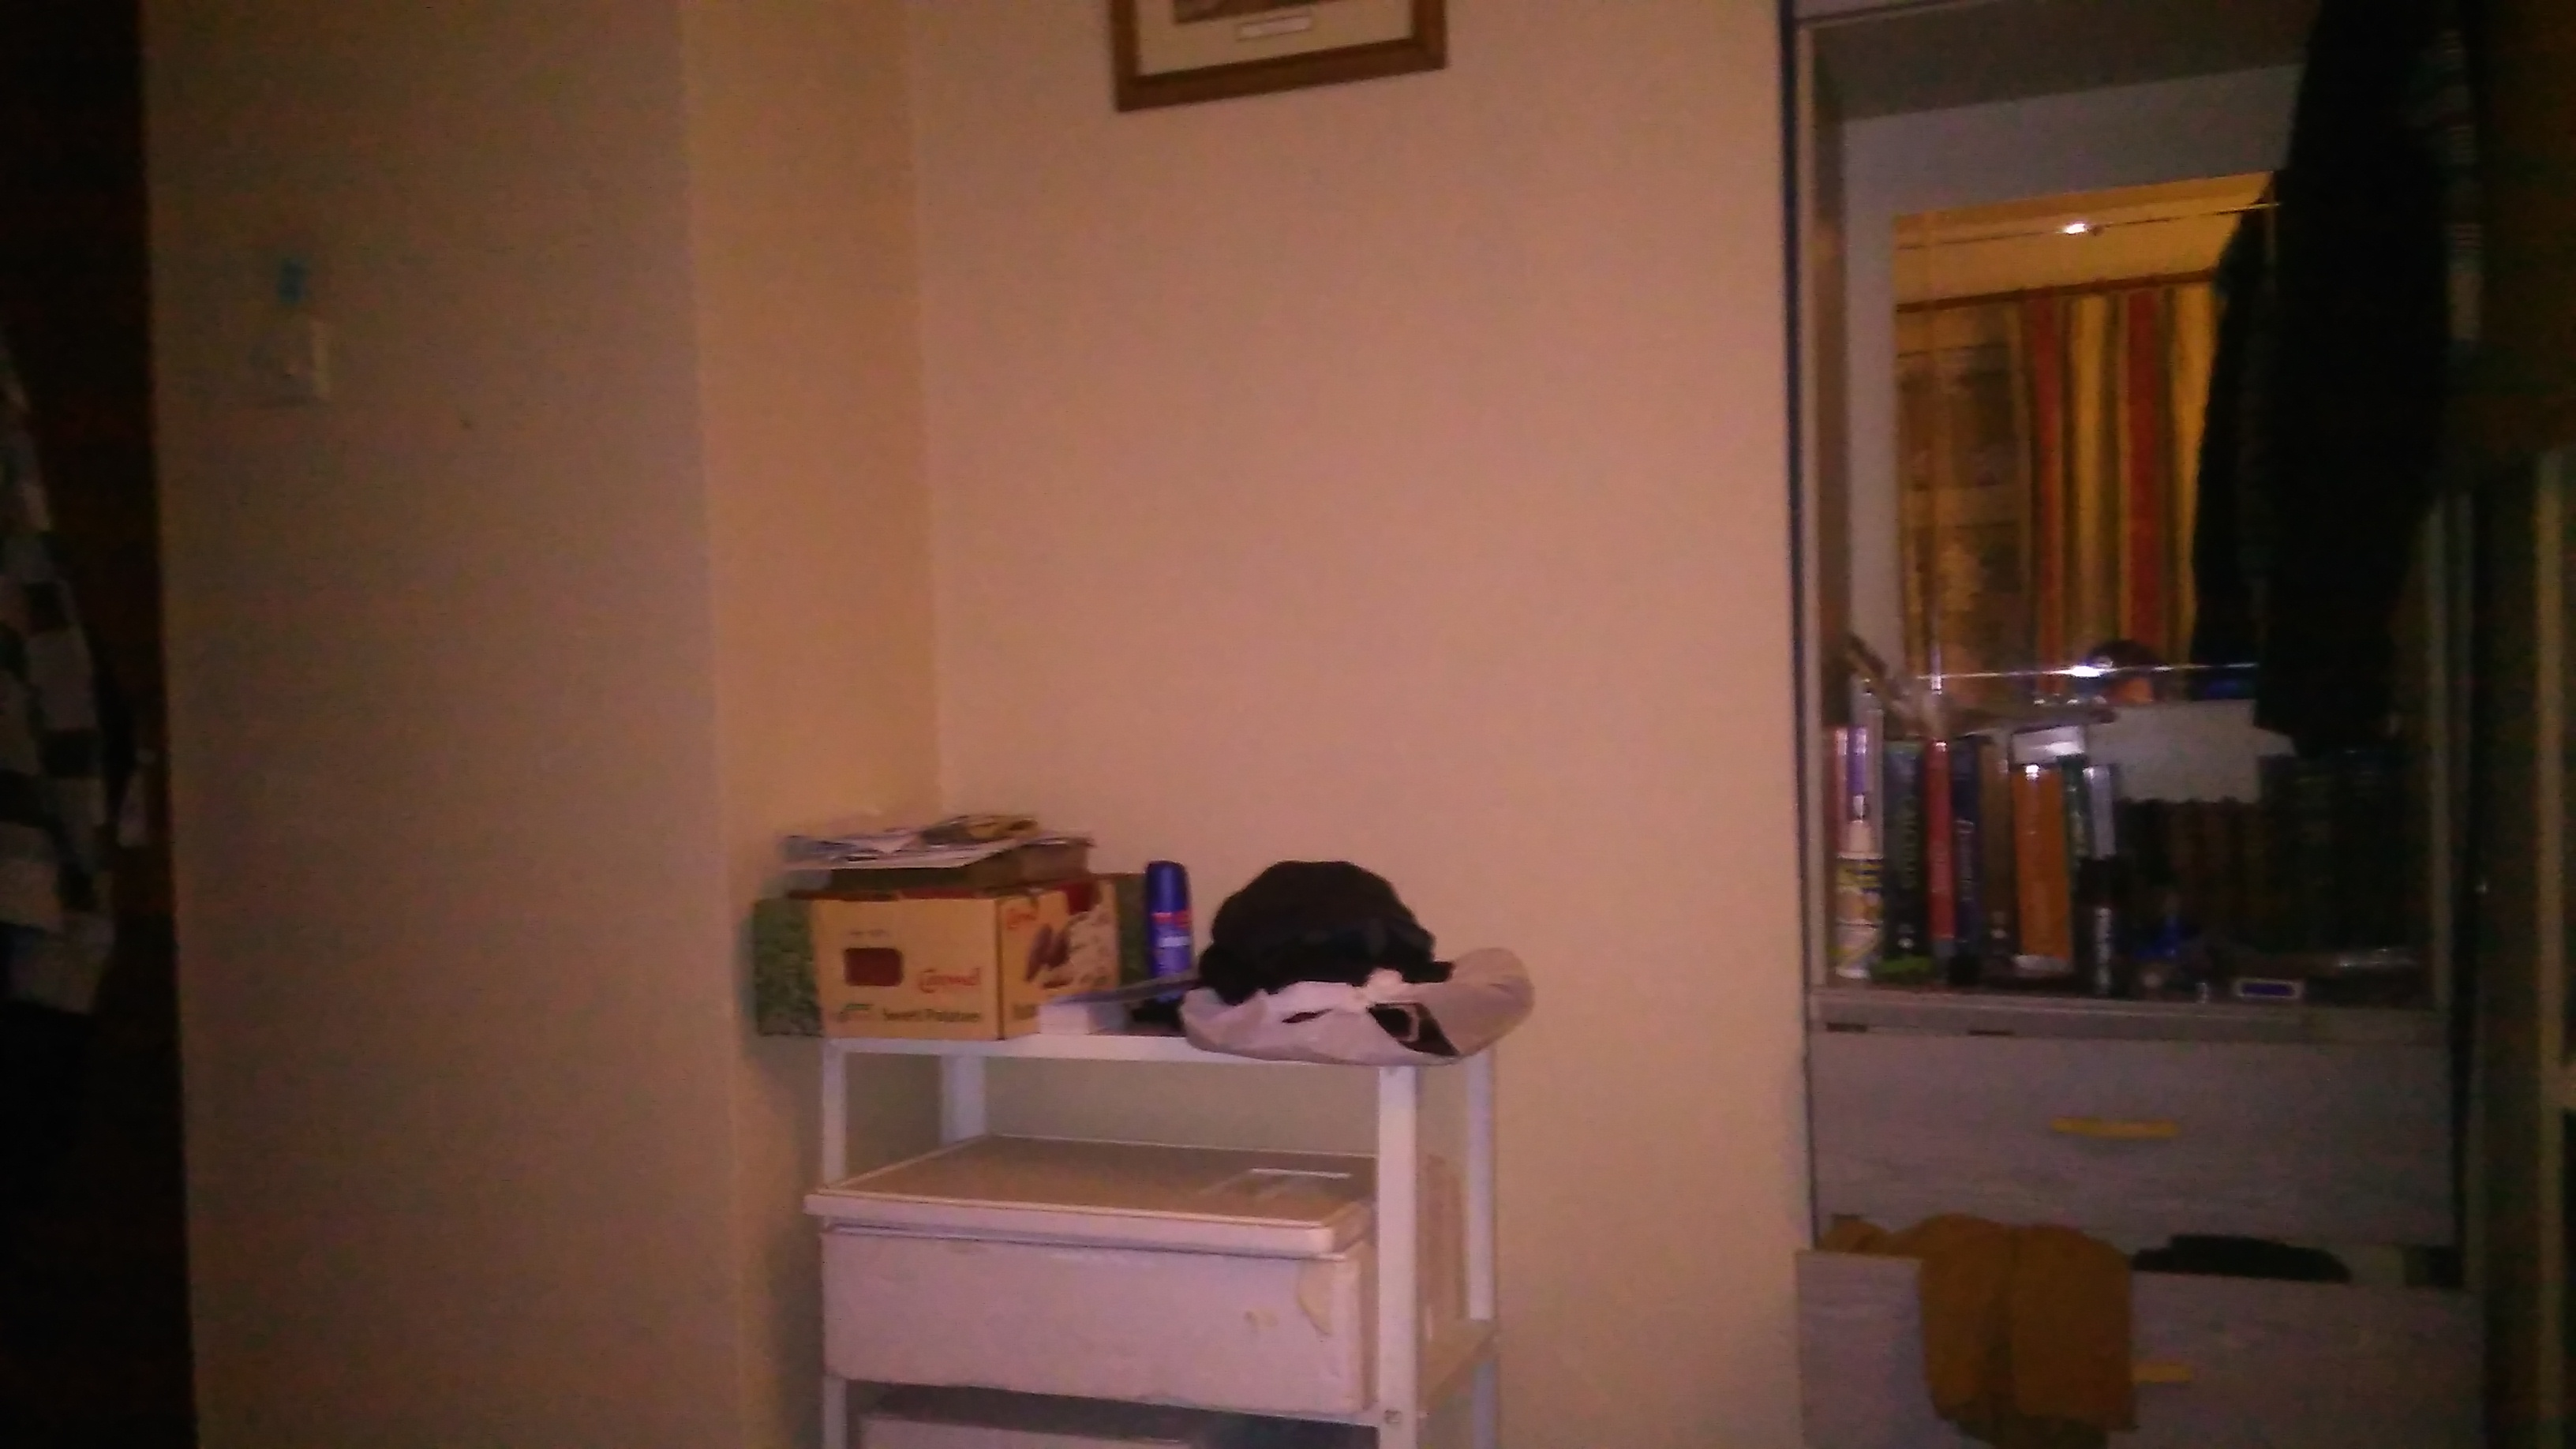
\includegraphics[width=8cm]{p1.jpg}
	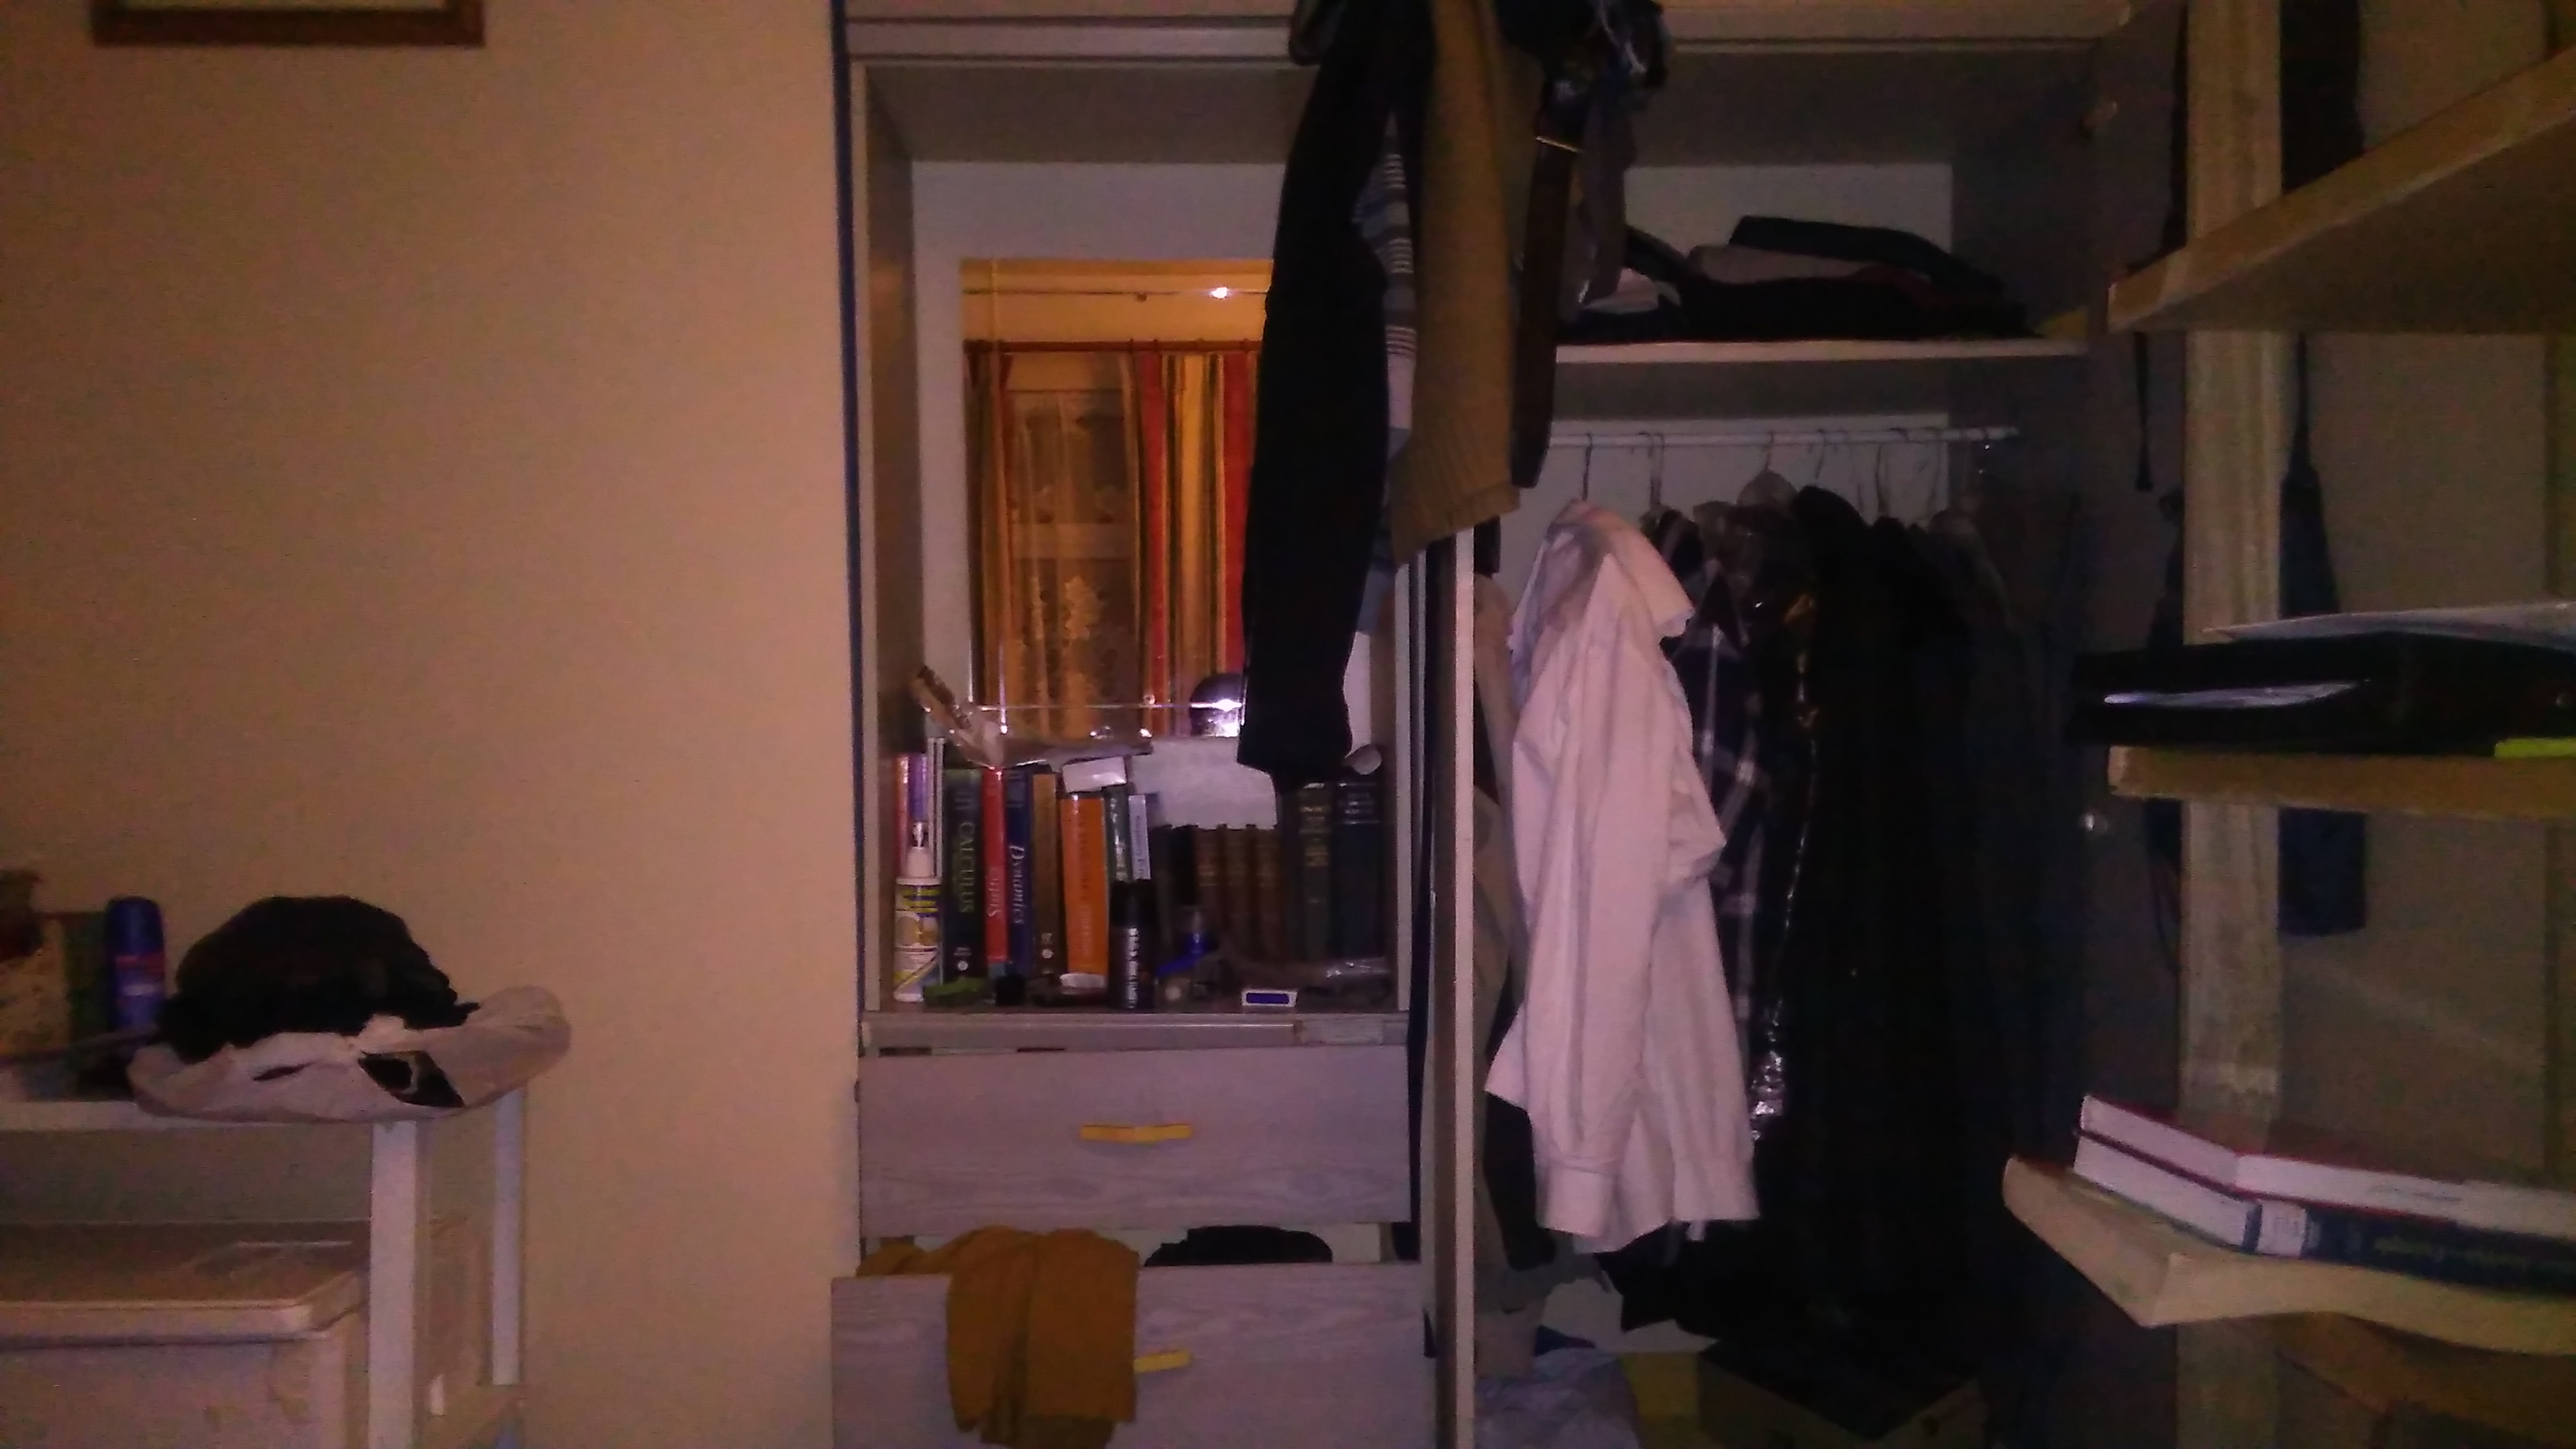
\includegraphics[width=8cm]{p2.jpg}

\end{figure}

Once the pictures are read in, feature detection along with feature matching and warping are performed on the pictures. This is to calculate if:
\begin{itemize}
	\item The images have features in common
	\item these features are numerous enough to perform panorama stitching
	\item If some of the images are warped to de-warp them, or if they require warping then to alternate them
	
\end{itemize}


\begin{figure}[H]
	\centering
	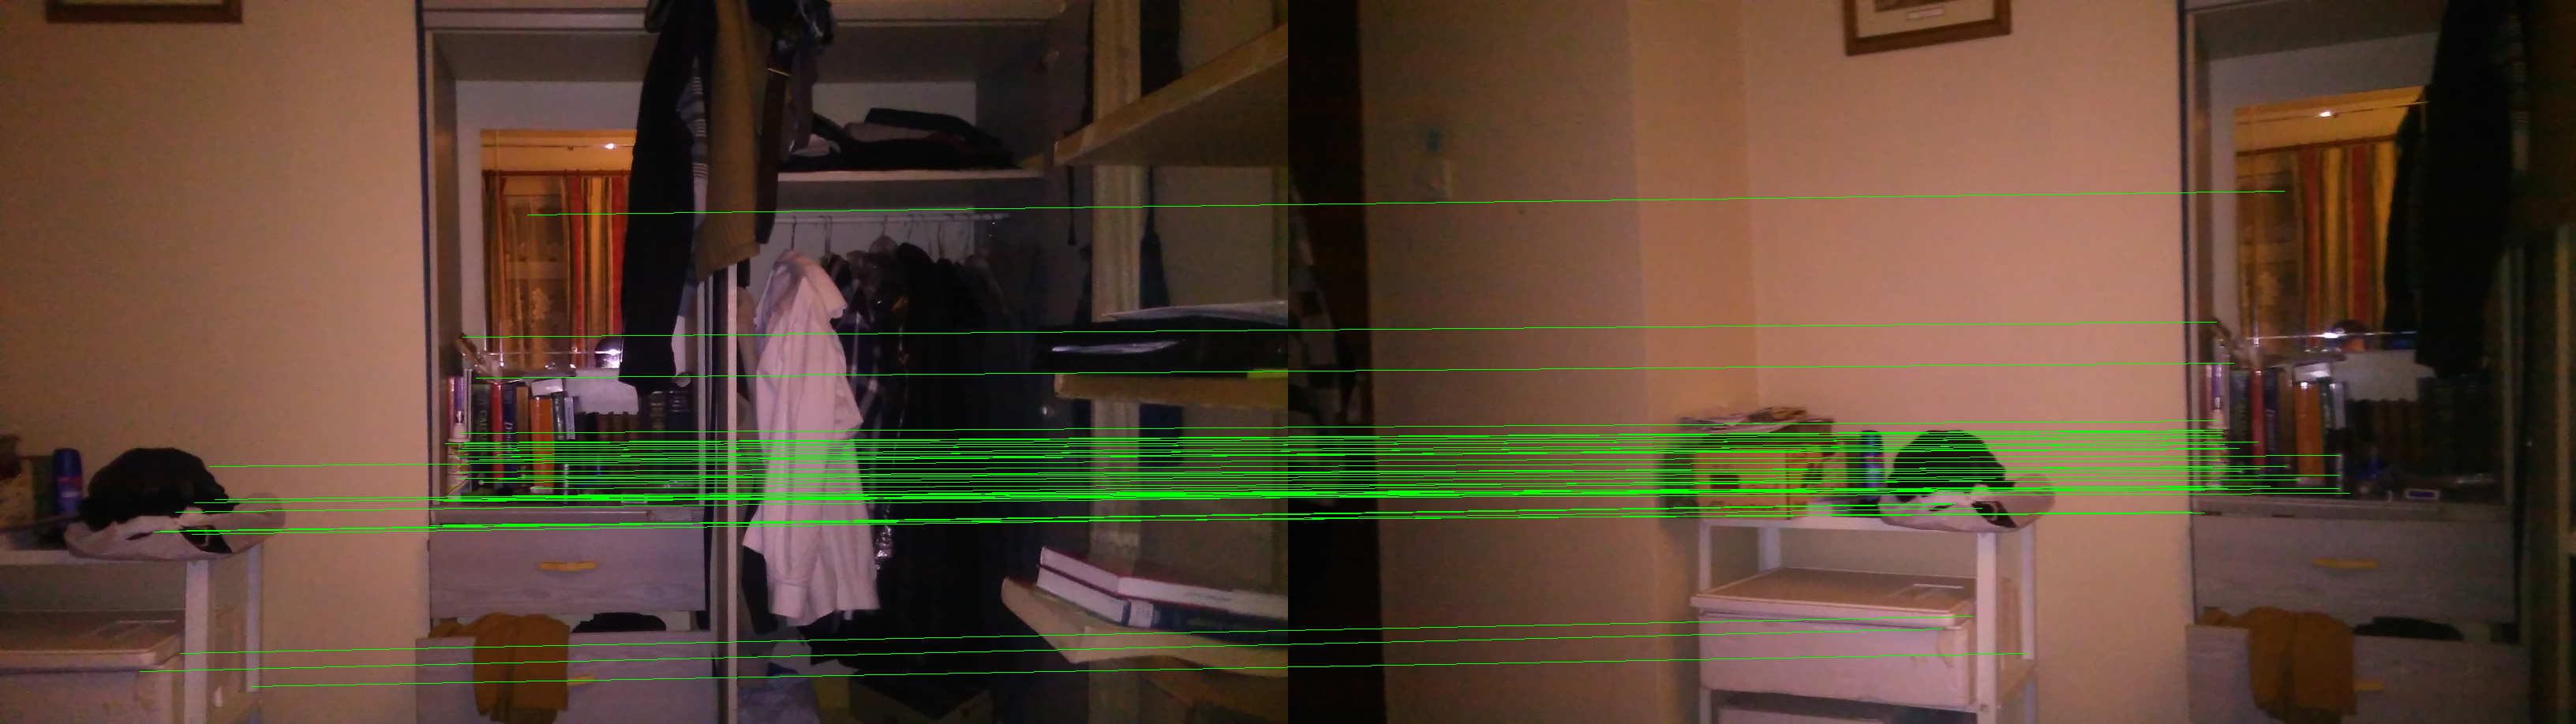
\includegraphics[width=14cm]{1v.png}
	
\end{figure}
The image above is of the two input images and the features which exist in both of them being connected with green lines.\\
As can be seen the lines only exist in the areas where the images overlap, as a line cannot exist where the features are not present in both images.\\
The only place where there are features detected however are in the books and clothes due to their asymmetric placing and color, the walls and large white spaces are not taken into account, even though they overlap. 
\begin{figure}[H]
	\centering
	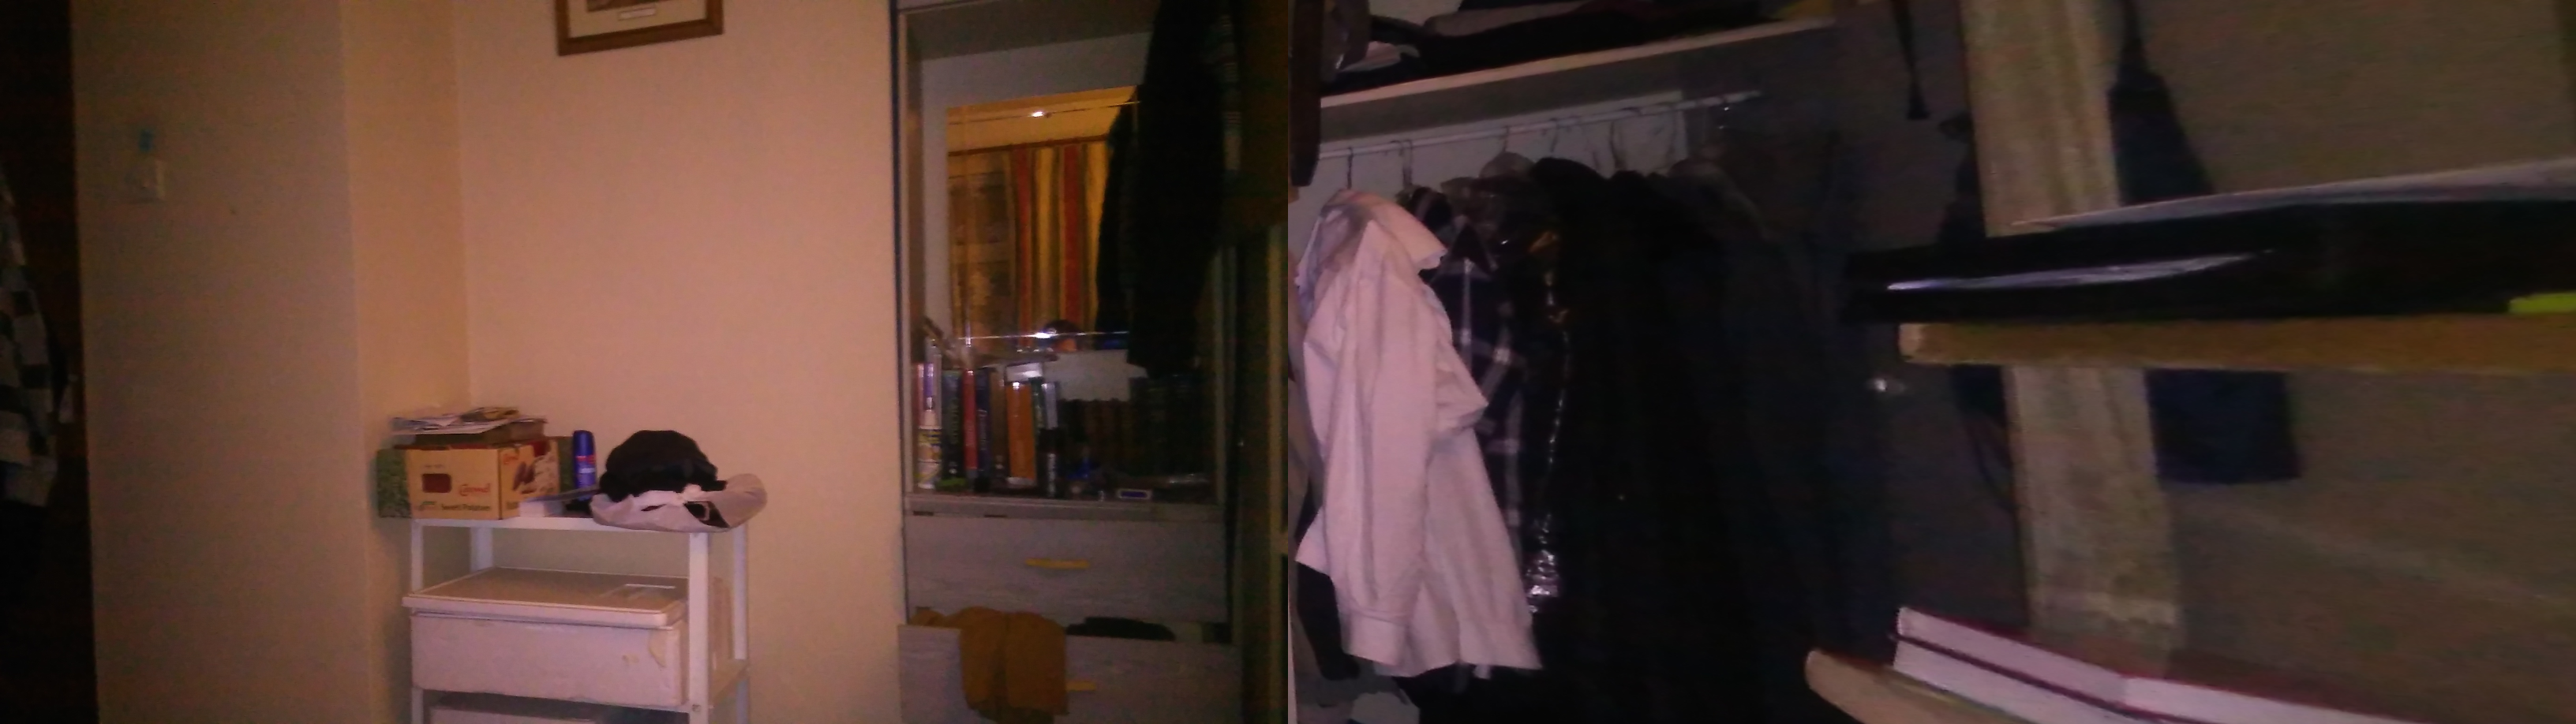
\includegraphics[width=14cm]{res2.png}
	
\end{figure}

Lastly the image above is the stitched panoramic image displaying  the features of both images.It can be observed that the right most image in the panorama ahas been warped to suit the spatial sense of the image. The image has enlarged bookshelves and a thinner door compared to the original.

\subsection{Part 2}\label{sec:overview}

The figures below show the real time panorama stitching from a continuous video. The video was taken off youtube and the stitching pipeline discussed above was followed closely to give this result. The video is not completely continuous but of comprised different segments taken throughout the day from a cold region. Therefore a completely continuous panorama from one video was not possible.\\
As long as the video was one continuous loop then the panorama can keep expanding, but once the loop breaks and another scene from a different location is displayed the panorama fails.\\
In theory a continuous panorama could be constructed if the frame rate of the camera were kept relatively low, the image quality was high and the camera moved through a distinctive scene at a steady page.\\
Otherwise the code can be used to stitch 2 or 3 or more multiple feeds from surveillance cameras as long as those frames overlap.

\begin{figure}[H]
	\centering
	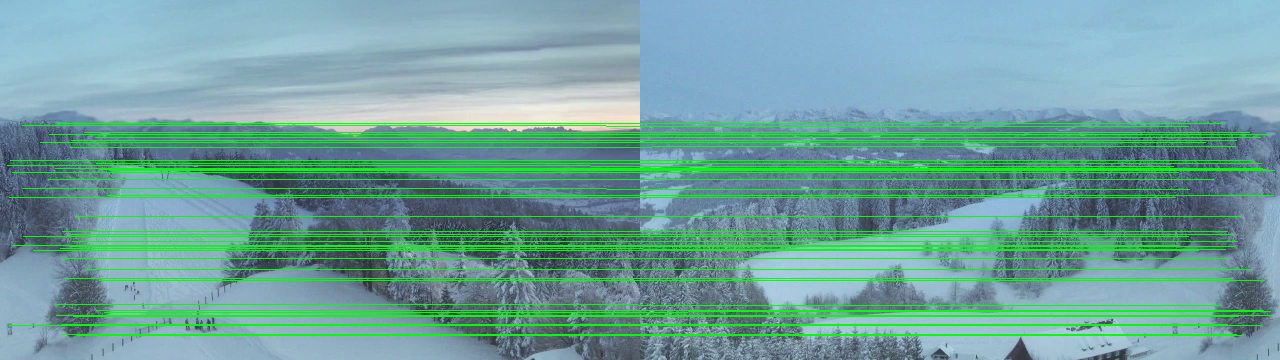
\includegraphics[width=14cm]{vpano.png}
	
	
\end{figure}

The only parts which opencv had a difficulty with stitching were the frames in which a timer or time stamp would arise. In these instances the time stamp would be copied across and the panorama would have 2 time stamps present instead of just the 1. This may be due to the fact that the time stamps are present in the exact locations and unlike the scenery do not move.
This can be attributed mainly to the fact that time stamps are generally in the bottom or top right hand corner, thus if the time stamp part of the frames does not overlap it leads the program into believing that there are 2 different time stamps.\\

 Therefore even though they are detected by the feature detection, they're immovable presence combined with the assumptions made by feature detections leads to opencv believing that they exist separately.

\begin{figure}[H]
	\centering
	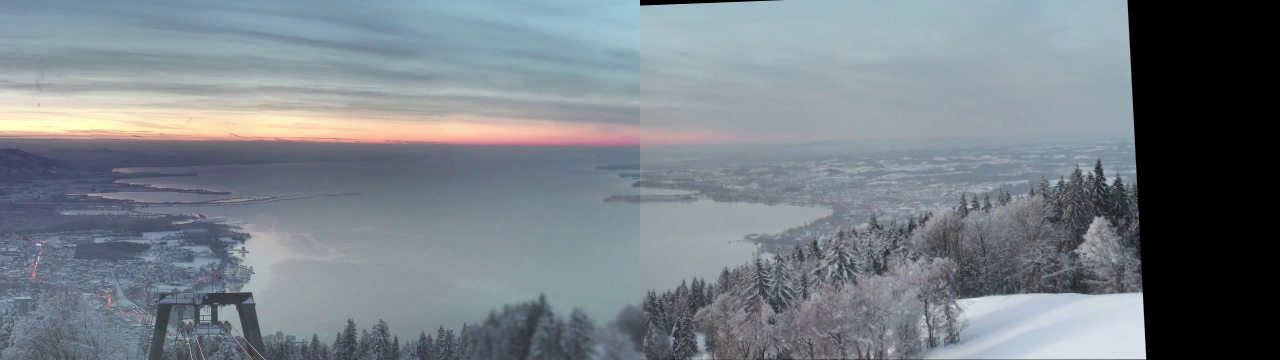
\includegraphics[width=14cm]{pano.png}
	
	
\end{figure}

\pagebreak
\subsection{Part 3}\label{sec:overview}

For the 3rd part of the code, two overlapping images were taken, to view the full example, these images needed a face in each image or possibly just one image.
Haar cascades were then used to detect if there were faces and eyes present in the frames and if so then overlay them with colored boxes. After the faces have been detected the images are taken through the stitching pipeline and a panorama with integrated face detection was constructed. 


\begin{figure}[H]
	\centering
	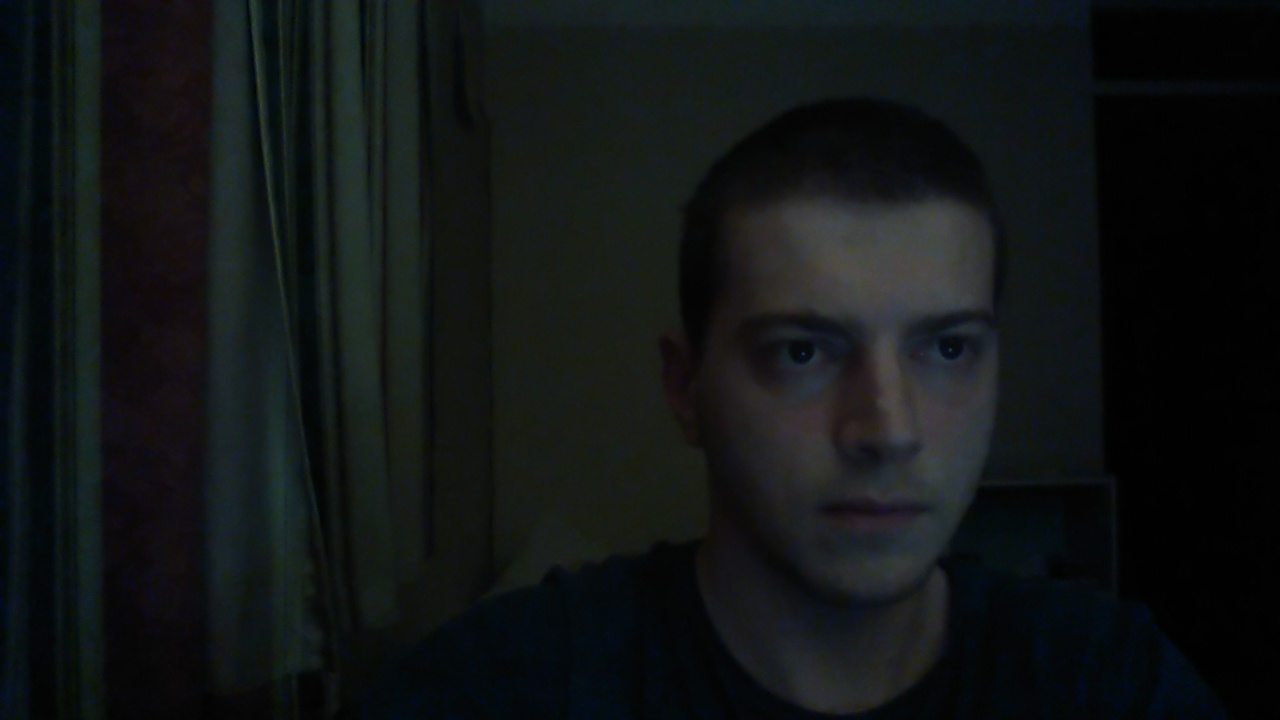
\includegraphics[width=8cm]{it1.jpg}
	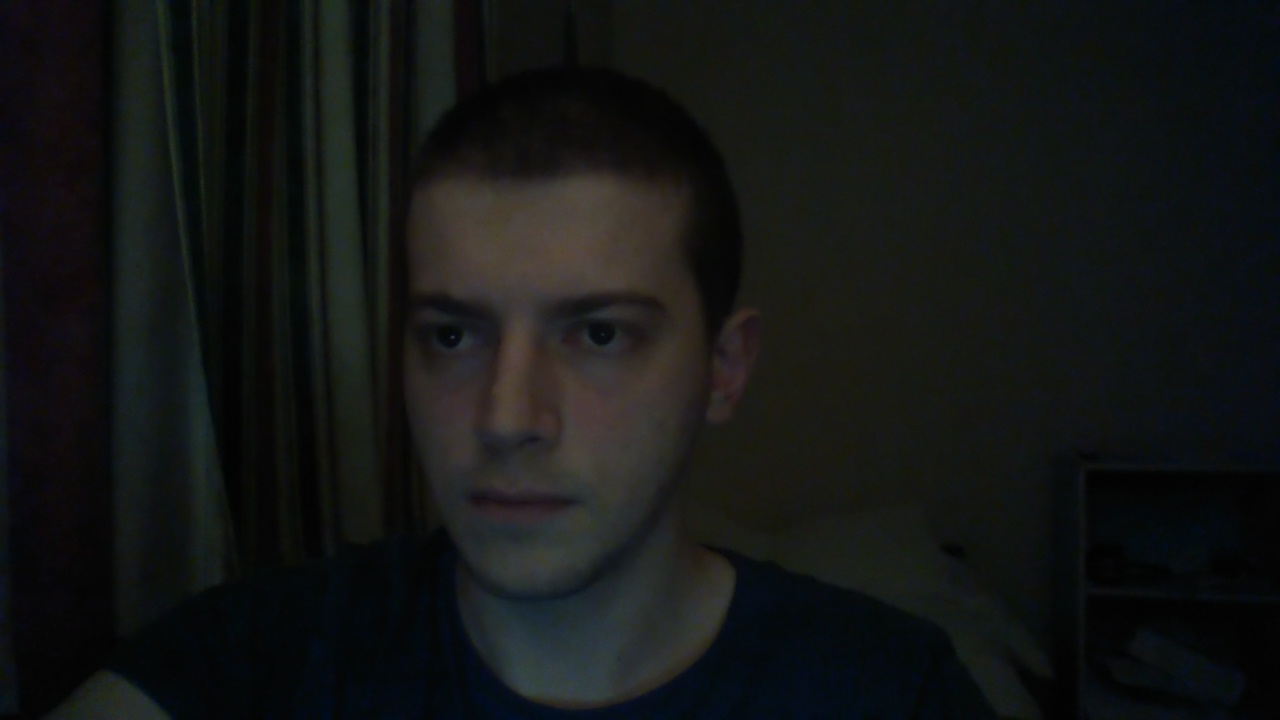
\includegraphics[width=8cm]{it2.jpg}
	
\end{figure}

\begin{figure}[H]
	\centering
	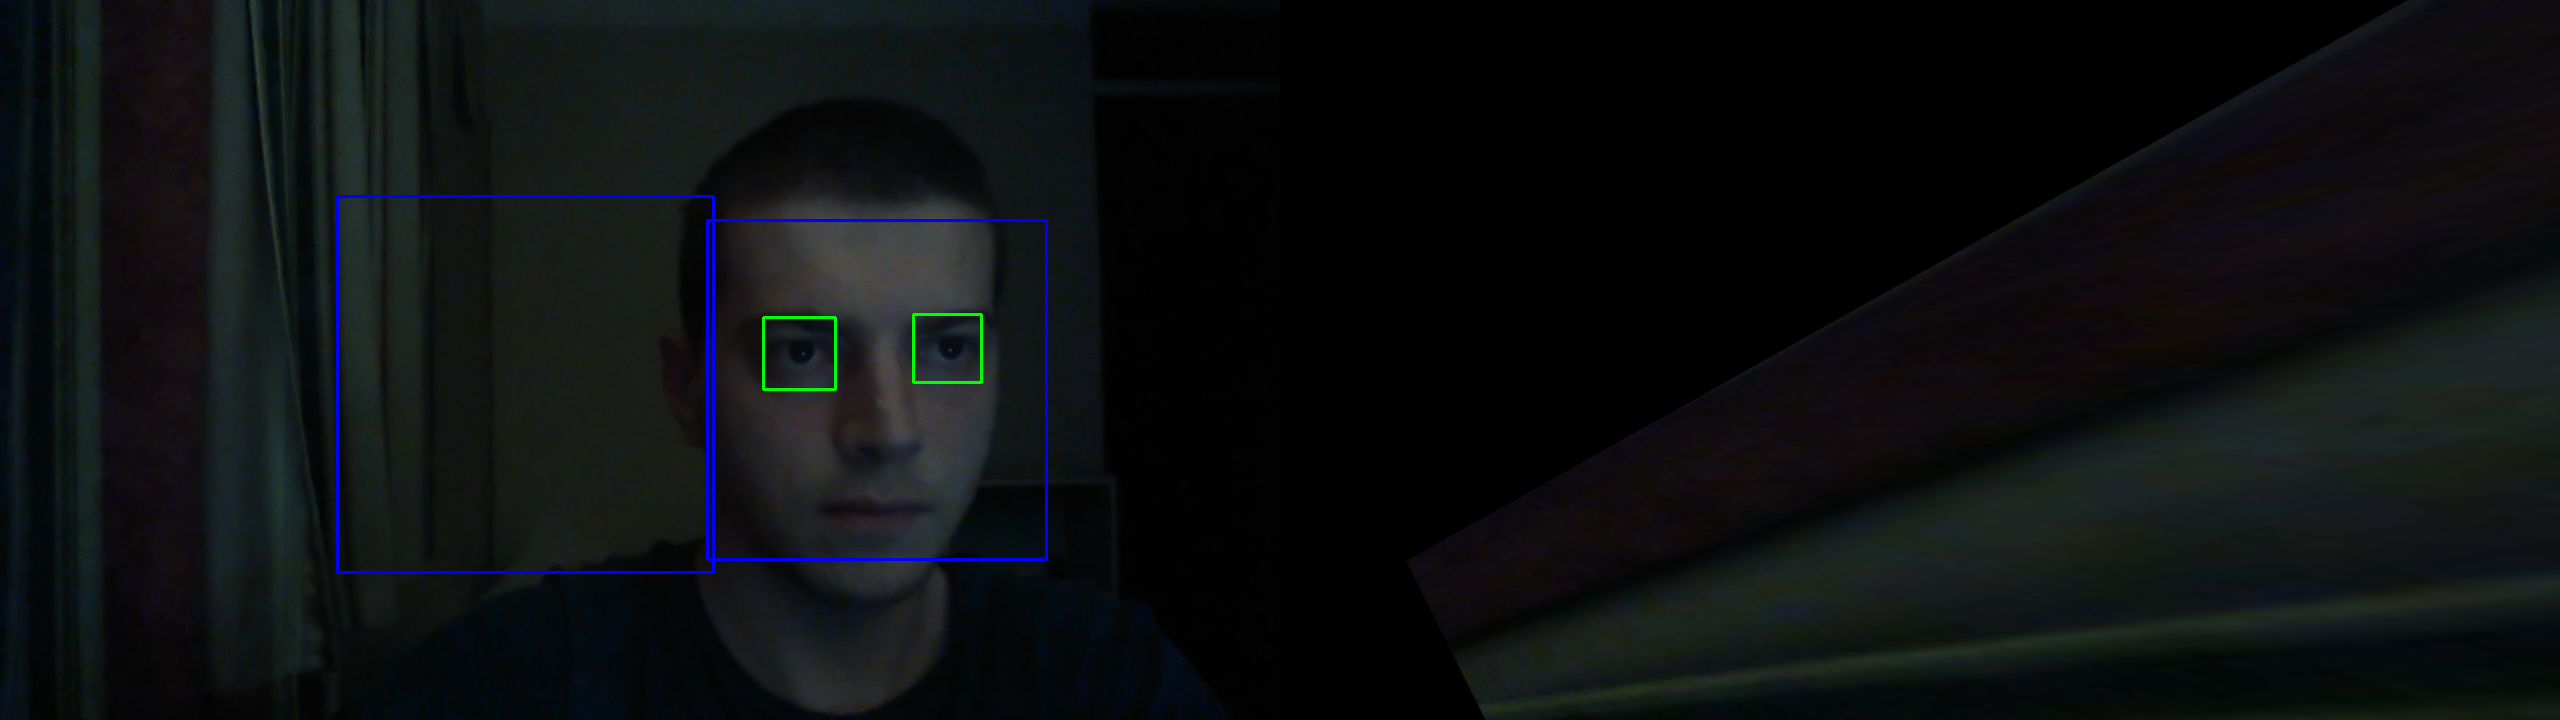
\includegraphics[width=15cm]{afce_pano.png}

	
\end{figure}

As can be seen in the picture below, the face detections and panoramic stitching have some small troubles when stitching images in low lighting conditions. This is due to the opencv packages struggling to detect features in such a featureless image. One thing which this image is missing is color and shape variance. Unlike the first stitching, these input images are void of vibrant colors and protruding angles on which opencv to detect features.
Therefore the warping aspect is somewhat thrown off. In proper lighting conditions and with more color in the frame the panorama could show better results.

\begin{figure}[H]
	\centering
	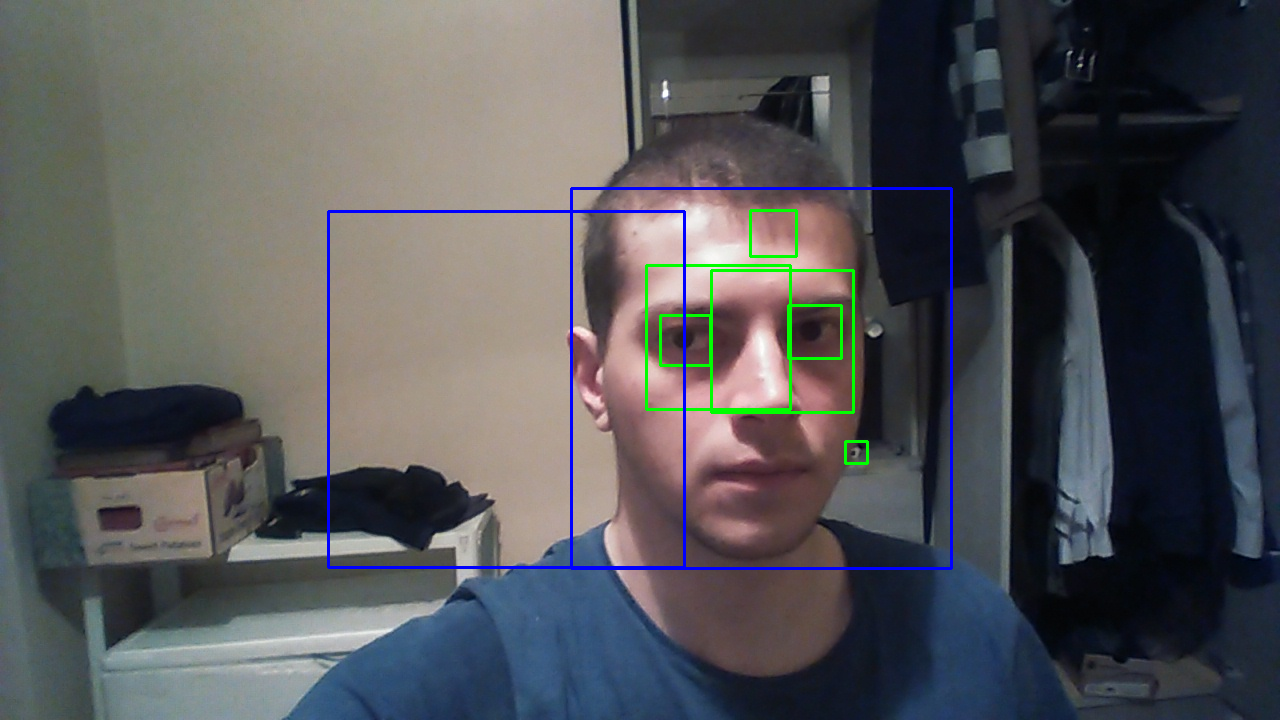
\includegraphics[width=8cm]{pk1.png}
	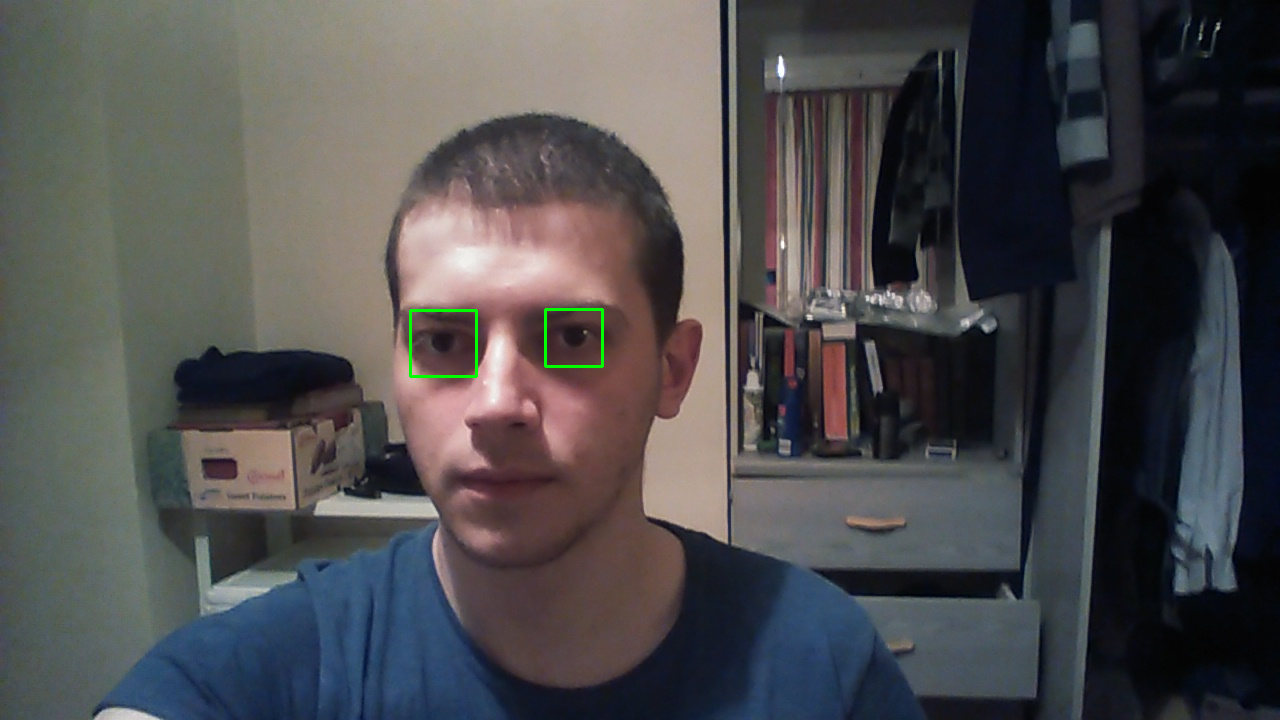
\includegraphics[width=8cm]{pk2.png}
	
\end{figure}

\begin{figure}[H]
	\centering
	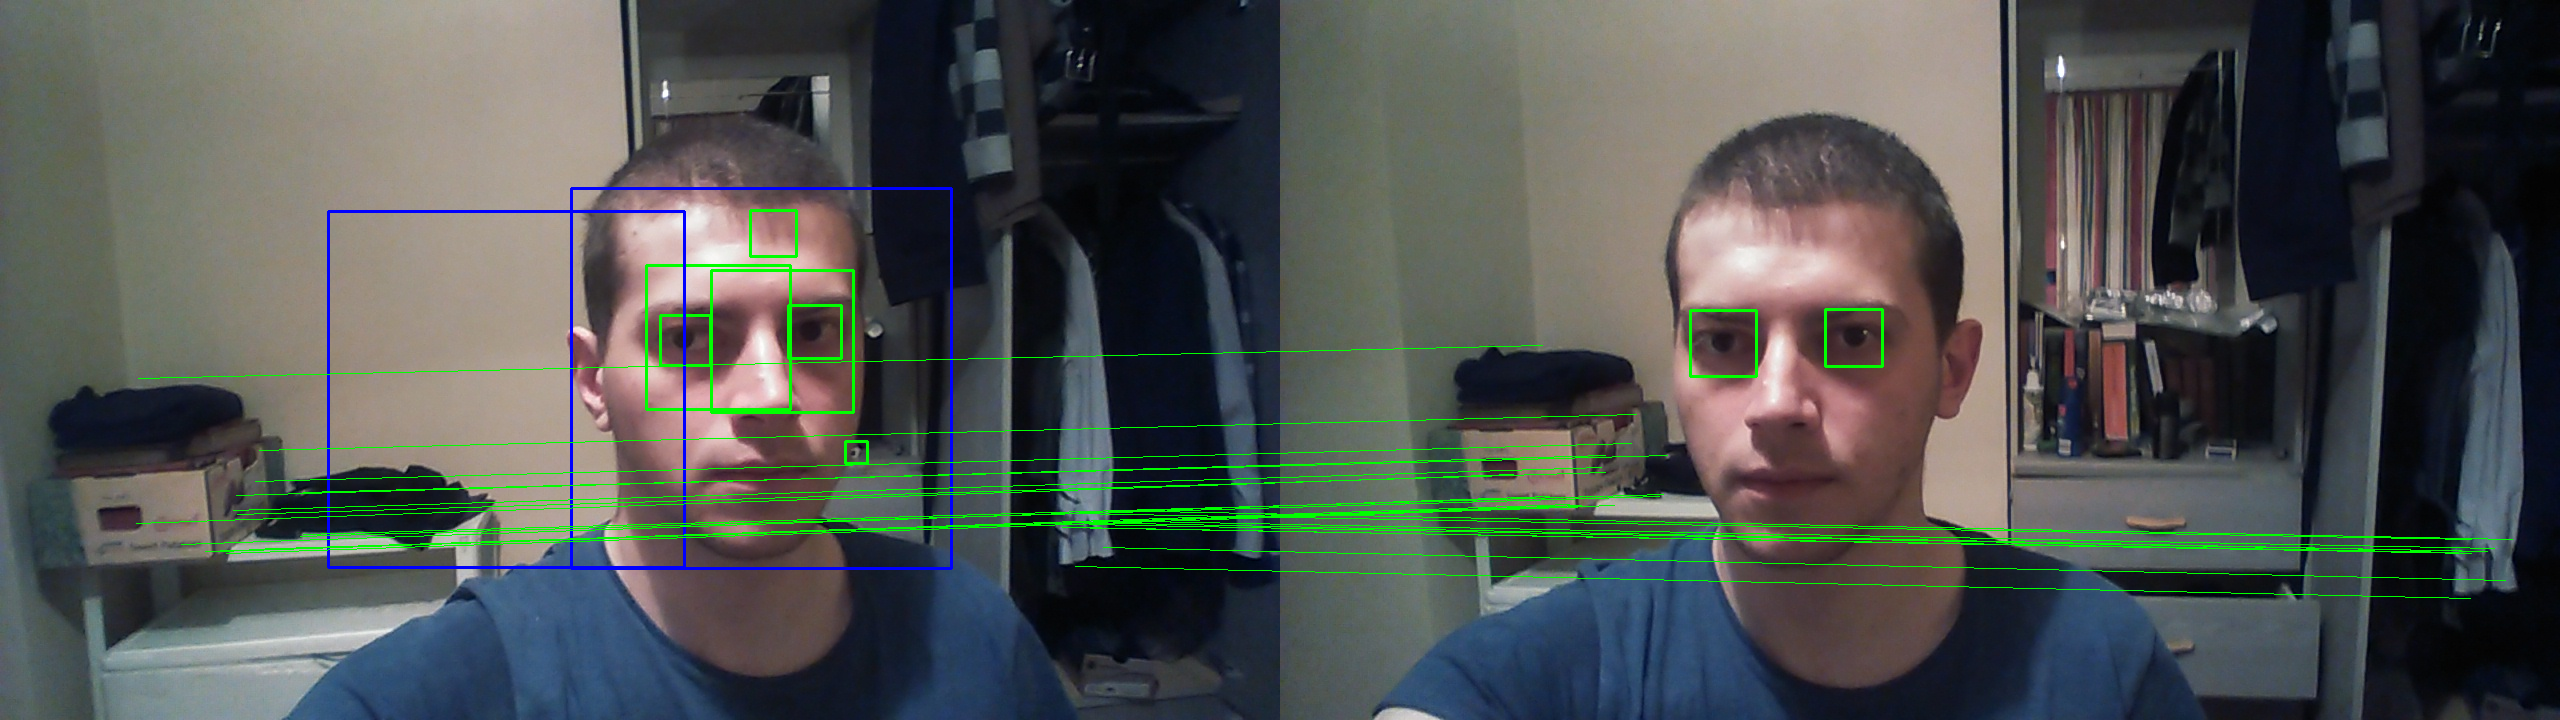
\includegraphics[width=15cm]{pkv.png}
	
	
\end{figure}
\begin{figure}[H]
	\centering
	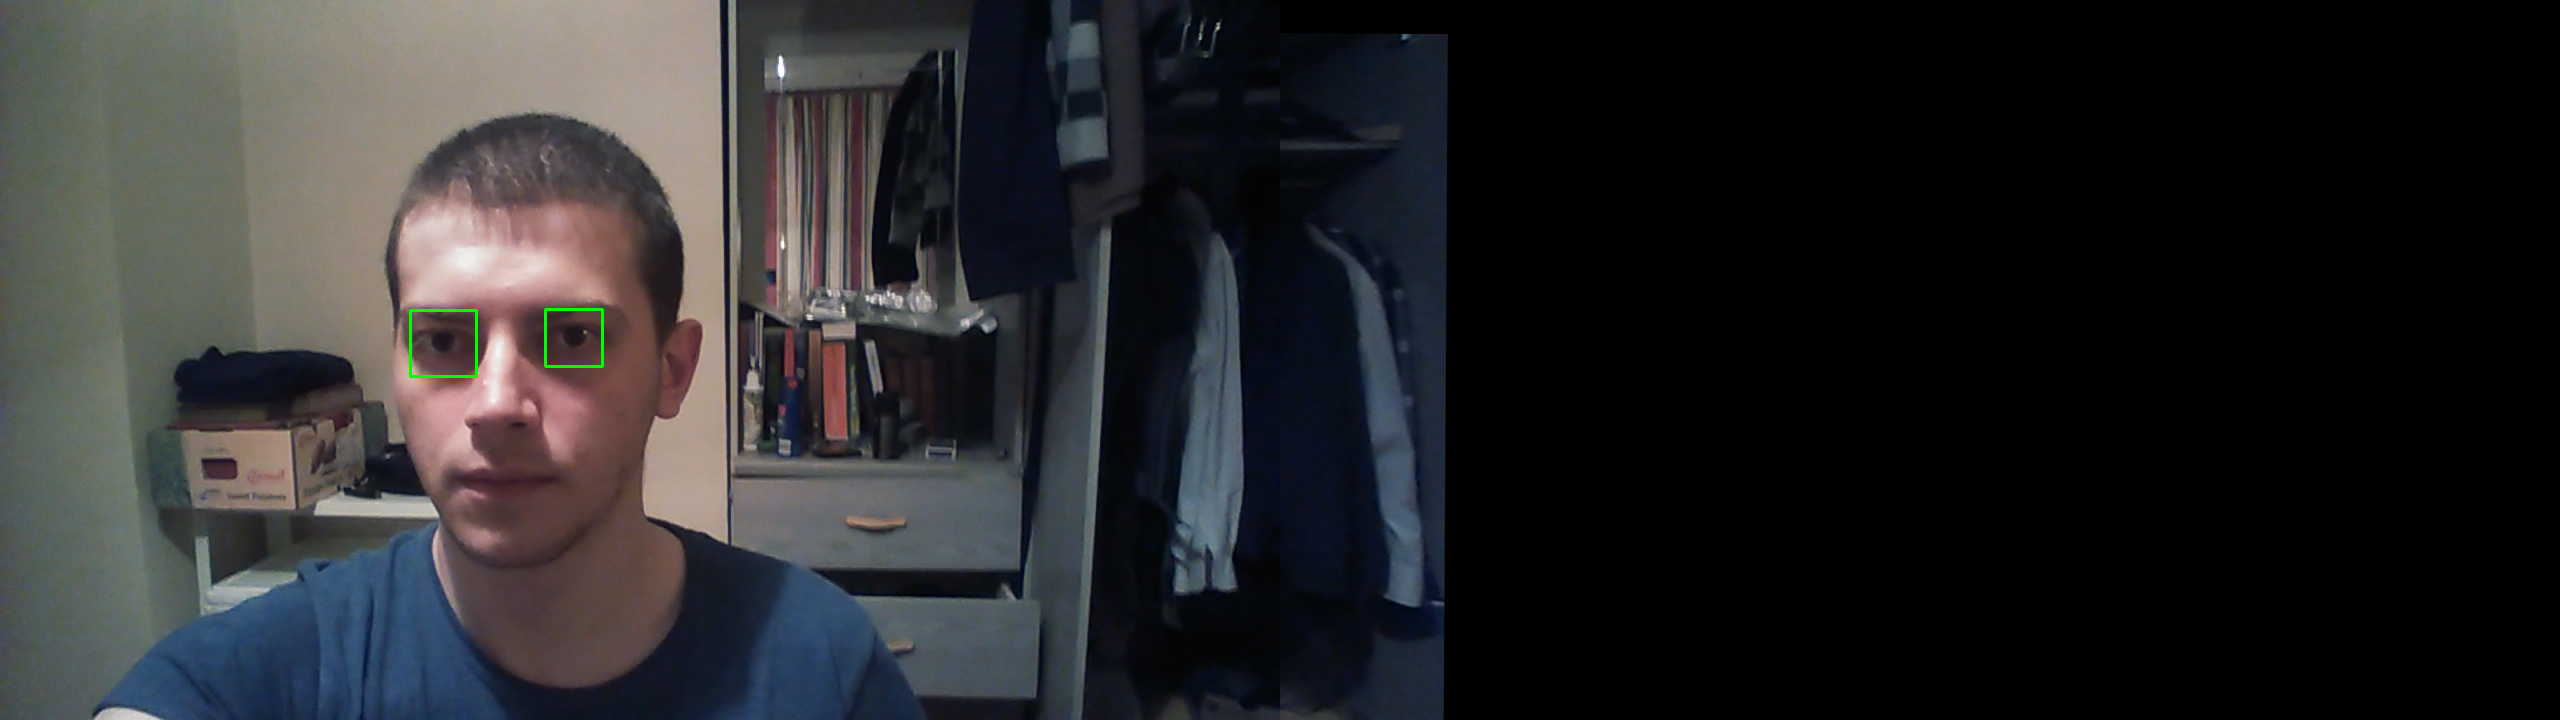
\includegraphics[width=15cm]{pkr.png}
	
	
\end{figure}
As can be seen in the above pictures, the overlap and lighting were severely increased and the image became more readable and thus a panorama was successfully produced.\\
Unfortunately there are not a lot of options in mitigating low lighting conditions. The only ones which are commercially available are infrared cameras which return gray scaled images in low lighting conditions or to use adaptive filters and canny to fish for features.\\
If money is available then the infrared camera option is always preferred, this however has a range limit of less than 100 meters and the quality of the images is also severely reduced.\\
Using canny is a lot cheaper than reinstalling all the hardware in a building. While cheap, canny has problems in variable light conditions and struggles to adapt across multiple frames. All that someone would need to blind all cameras in the vicinity would be a bright blinking LED.
Lastly it can be seen that since only one frame had face detection, then the panoramic pipeline resulted in dropping all the features which did not exits in both images, this being everything but the eye detection. Thus to conclude, face detection would be far more reliable if performed after panorama stitching so as to avoid loosing data later on.

\pagebreak
\section{Summary}\label{sec:overview}
\begin{wrapfigure}{L}{0.3\textwidth}
	\centering
	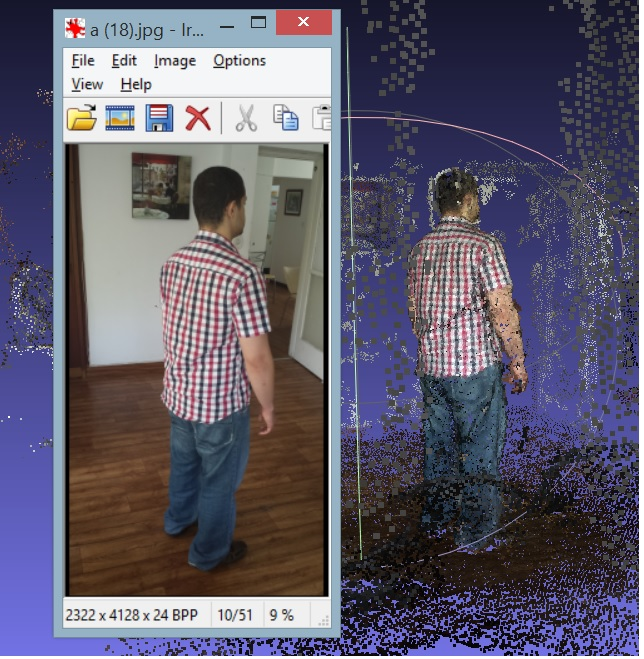
\includegraphics[width=5cm]{reconstruction2.jpg}
	\caption{https://gilscvblog.com/2014/05/15/an-easy-and-practical-guide-to-3d-reconstruction/}
\end{wrapfigure}
It has been found that there needs to be a certain amount of similarities between the images for stitching to be possible, otherwise the image stitching fails. Through a variety of experiments and online research, it is generally agreed among the opencv community that at least 4 similarities must be found between 2 images to qualify as valid candidates for panorama stitching.\\

The last part of the project involved taking the images and constructing a 3d panoramic representation of a scene. This was however unsuccessful due to the vtk package needed to draw in 3d not being able to work with the virtual environment or the normal environment.


The majority of the time was spent mainly with cmake and various libraries in getting them to work. This is due in a large part ot how opencv3 now works. Due to legal conflicts, many of the functions which were easily accessible in opencv2.4 are now significantly harder to access. This causes an added dimension of anxiety as each system setup and language wrapper is different. For this project I have attempted to perform image stitching across all 3 platforms.\\
The windows  packages for opencv\_contrib are mainly abandoned since 2012, the information pertaining to this is however extremely difficult to find. Due to the lack of support for windows, the packages will not work on windows 10 and thus a pirated version of windows is needed as windows 7 is no longer openly distributed or sold. \\
Secondly MACOS is a lot easier to run opencv initially, it too however does no longer have support for vtk since 2012. Siearra as of now is not supported to run any of the non-free opencv\_contrib packages.\\
Ubuntu 16.04 opencv3 is the most if not only up to date package for running opencv\_contrib non-free algorithms.\\

Due to not knowing this, a large amount of time was lost finding the most compatible operating system.\\
The project was firstly written in c++ but was then migrated to python 3.5. This choice was made solely on how much more easy it is to import packages in python rather than in c++. For example the c++ opencv3 packages would require that an include was specified for every file, where as in python all is needed is import cv2.\\
One drawback of using python was the lack of support as opposed to c++ for opencv. The packages seem to be structured based on language and the python distribution does not have some critical stitching functions present in c++. This is where the stitching pipeline in python becomes more manual than that in c++.\\

The stitching pipeline was almost completed to reach all the goals set out. The last part which would have been the most interesting would have been to not only create a panorama from video, but also a 3d model representation panorama of the frames extracted from the video. To draw in 3d space, vtk is needed to work with opencv3. Opencv extracts the points from the 2d images and if the frames intersect and meet the stitching requirements, then not only could a panorama be stitched, but also 3D points be deduced from the images. The 3d points would then only need to be drawn in 3d space with the corresponding color of the points.\\




The code for all the processing was present, but vtk could not be integrated with all the opencv packages in time for this project. It is however a very interesting project which I wish to finish later on. 
As for the panoramic stitching, it was interesting to not only understand how the panorama pipeline functioned but also to see it applied in c++ and python and to explore the strengths and weaknesses of each implementation. \\
To conclude, panoramic image processing requires a lot of theoretical understanding but also checks and double checks in the code implementation.Anything from low/high lighting conditions, video time stamps and distorting objects to out of angle frames can completely ruin a panoramic shot.


\section{Video}\label{sec:overview}
https://youtu.be/ysWWgZUdov0



\cleardoublepage
\bibliographystyle{IEEEtran}
\bibliography{/Users/admin/Desktop/LAB_REPORTS/security/aug/references/references.bib}
\end{document}



